\startchapter{Real-time Cutting}
\label{chapter:Cutting}
One of the main objectives of virtual reality based surgical simulation systems is the removal of pathologic tissue 
\cite{Steinemann, Nienhuys2001a}. Cutting imposes many challenges in the development of a robust, interactive surgery 
simulation, not only because of the nonlinear geometric and material behavior exhibited by soft tissue but also due to the
complexity of introducing the cutting-induced discontinuity. In most publications, the progressive surgical cutting is modelled
by conventional finite element (FE) method, in which the high computational cost and error accumulation due to remeshing constrain 
the computational efficiency and accuracy. 

We developed our new cutting approach in the context of brain biopsy simulation. When an abnormality of the brain is suspected, 
Stereotactic (probing in three dimensions) brain needle biopsy is performed and guided precisely by a computer system to avoid 
serious complications. A small hole is drilled into the skull, and a needle is inserted into the brain tissue guided by computer-assisted 
imaging techniques (CT or MRI scans). Due to this, the actual cutting process can not be seen by the surgeon. For this reason,
non-progressive cutting, where a tetrahedral element is decomposed only once is has been completely traversed, is a reasonable
approximation for our application area, and so we define the cut only once the instrument has traversed the pathology. 
Moreover, there is little, if at all, resistance to the cut tool movement through the tissue. Therefore, in the current stage, we do 
not model any interaction of the cutting tool with the deformable object during a cut. 

The deformable tissues in our framework are represented by tetrahedral meshes and simulated using nonlinear finite element methods. 

\section{Related Work}
A number of approaches has been proposed by the computer graphics community to enable cutting deformable models. 
Except for a few methods most of them used tetrahedral meshes for the volumetric mesh representation. 
Bielser \etal performed an adaptive refinement of the tetrahedral elements cut by a virtual scalpel \cite{Bielser1999}.

Mor \etal tried to reduce the number of sub-elements created while cutting tetrahedral meshes \cite{Mor2000}.
One of the major issues in cutting is the creation of ill-shaped elements i.e. skinny elements, which can adversely affect the
performance and stability of the system solver. Some works attempted to avoid such elements via mesh alignment techniques 
\cite{Nienhuys2001a, Steinemann2006}. Other methods tried to solve the issue by removing them completely.

Jin \etal proposed a meshless total Lagrangian adaptive dynamic relaxation cutting algorithm to predict the steady-state 
responses of soft tissue \cite{Jin2013}. A cloud of points is used for discretization and approximation of the deformation 
field within the continuum without generation of finite element meshes. They didn't report 
any performance measurements and the quality of the cuts could not be verified with the simple truth cube model they reported in their paper.
 
Wu \etal \cite{Wu2011} proposed an algorithm for 3D mesh cutting using a combination of the adaptive octree refinement with iterative composite
element hierarchy to enable simulating high-resolution cuts with a small number of degrees of freedom (DOFs). 
They used the dual contouring method \cite{Ju2002} to keep the sharp creases along the cut. Due to the high computational cost and naive implementation 
their method is not scalable and has yet to become an interactive cutting approach.

In a closely related work Courtecuisse \etal presented a soft-tissue cutting system with haptic 
feedback \cite{Courtecuisse2010a}. Their cutting strategy follows Mor \etal  \cite{Mor2000} work and 
suffers from jaggy lines along the cut surface as shown in their examples of a laparoscopic hepatecotomy.
The progressive is not supported in their system and as most of the other works in this area they produce too many
new nodes when subdividing cut elements.

Jerabkova \etal proposed a solution to ill-shaped elements problem by using hexahedral elements instead of 
tetrahedra \cite{Jerabkova2010}. Their approach relies on fine-level voxels to model object surface and simulate cutting. 
The volume data requires more memory space than traditional, surface-based models. Cutting is performed by
removing voxels. For sufficiently small voxels this typically remains unnoticeable but it may result in 
significant volume loss in case of a large number of cuts. 


Sifakis \etal \cite{Sifakis2007} proposed a geometric algorithm for placing cracks and incisions on 
tetrahedralized deformable objects. Their method is similar to the virtual node algorithm in that they avoid 
sliver elements and their associated stringent timestep restrictions. Producing ill-conditioned triangles on 
the material surface can have a negative effect on collision handling specially in case of a self collision.
Also in their system a cut that partially intersects a tetrahedron without separating it into disconnected 
fragments will not allow the material to separate within that embedding tetrahedron.

Steinemann \etal \cite{Steinemann} created a hysteroscopy simulator and minimized the number of added elements 
after a tetrahedral subdivision by cutting along existing edges and faces. The problem with their system is that
they model the result of the cut only after it has been completed and this leads to felt lag in the response
of the system. Unfortunately they didn't report any performance statistics of their system. 

In the following sections we provide an overview of the system, the data structures involved in the process 
and our cutting algorithm. The chapter is concluded by analysis of some simulation results.

\section{Overview}
We present a GPU-assisted approach in cutting tetrahedral meshes in real-time. 
The input to our system is a cut trajectory and a half-edge data structure representing the tetrahedral mesh. 
The following steps are carried to complete the cut induced by the scalpel on the mesh:

\begin{enumerate}
 \item Using the cut trajectory and the bounding box of the cutting tool, the sweep-surface that passes through 
 the mesh is defined.
 \item Using the GPU-accelerated algorithm the intersection of the sweep-surface and all the edges of the mesh 
 are computed. The output of this stage is a list of cut-edges and their associated intersection points. 
 
 \item A GPU kernel function is used to compute the distance of the nodes in the cut-edges and the end points of 
 the cut tool. This way the nodes that are close to the sweep-surface are identified and a different configuration 
 is used to produce subdivided elements in the next stage to avoid ill-shaped elements. The output of this stage is an
 associated list of cut nodes.
 
 \item Using a look-up table all the cut tetrahedra are decomposed into sub-elements
 
 \item The nodes identified to be close enough to the cut trajectory are snapped to the sweep surface
 
 \item The solver system is synchronized with the latest mesh changes, all the mass, damping and stiffness 
 matrices are updated.
\end{enumerate}


\section{Data structure}
The tetrahedron is the three-dimensional case of the more general concept of a Euclidean simplex. 
Figure \ref{fig:tetconfig3} shows the structure of a tetrahedral element and the order we chose to 
name the nodes, edges and vertices in its canonical orientation. In this figure $P_0$ to $P_3$ are
the vertices, $e_0$ to $e_5$ the edges and $F_0$ to $F_3$ are the faces of the element.

\begin{figure}[H]
  \centering
  % the following command controls the width of the embedded PS file
  % (relative to the width of the current column)
  \includegraphics[width=1.0\linewidth]{figures/cutting/tetconfig3.png}
  \caption{\label{fig:tetconfig3}
  {A tetrahedral element in its canonical view. Iterating over nodes, edges and faces of each element is
  one of the primary operations in a geometric algorithm that manipulates such elements.}
}
\end{figure}


In a complex mesh of tetrahedral elements accessing each of these components is a necessary requirement for 
implementing any geometrical algorithm. Therefore the main module in our cutting algorithm is a half-edge 
data structure that maps tetrahedral elements to their associated faces and the faces to their associated half-edges and nodes. 

The minimal set of operations frequently used by most algorithms are as following \cite{Mario2010PolygonMesh}:

\begin{itemize}
 \item Access to individual vertices, edges, faces and tetrahedral elements. This includes the enumeration of 
 all elements in unspecified order.
 \item Oriented traversal of the edges of a face, which refers to finding the next edge (or previous edge) in a face.
 With additional access to vertices, for example for rendering of faces if enabled.
 \item Access to the incident faces of an edge. Depending on the orientation, this is either the left or right face in the manifold case.
 This also enables access to neighboring faces.
 
 \item Given an edge access to its two endpoint vertices.
 
 \item Given a vertex, at least one incident face or edge must be accessible. 
 
 \item All incident face and edges in the so-called one-ring-neighborhood of a vertex can be enumerated.
\end{itemize}


\begin{figure}[H]
  \centering
  % the following command controls the width of the embedded PS file
  % (relative to the width of the current column)
  \includegraphics[width=0.8\linewidth]{figures/cutting/halfedge.png}
  \caption{\label{fig:halfedge}
  {Half-edge data structure to store mesh information. Each half-edge holds references to its previous and next half-edges,
  left and right faces and the two end points. It may also store a pointer to its opposite half-edge.}
}
\end{figure}

Per each node we also store the rest position of it, this is used to update the physics model and to interpolate the position 
of newly added nodes in case of cutting. To make the matters simple the two half-edges between a pair of nodes are stored 
consecutively in the mesh storage. This way the index of an edge is simply half of the index of one of its incident half-edges. 
To provide convenient access to half-edges and faces using their incident nodes, we used a hash map structure
which maps a pair of node indices to their associated half-edge index. For faces since needed to have unique faces between 
any given combination of three nodes we compute the hash key as following:

\begin{algorithm}[H]
\caption{Unique face key computation.}
\label{alg:facekey}
\begin{algorithmic}[1]	
  \STATE $nodes = fetchNodes(face)$ 
  \STATE $nodes = sort(nodes)$
  \STATE $bitmask = 0x001FFFFF$
  \STATE $key64 = nodes\left[ 0 \right] \And bitmask$
  \STATE $key64 += (nodes\left[ 1 \right] << 21) \And bitmask$
  \STATE $key64 += (nodes\left[ 2 \right] << 42) \And bitmask$
  
\end{algorithmic}
\end{algorithm}

Using the technique shown above we can address up to $2^{63}$ faces uniquely. The half-edge keys are computed using the indices to
the two endpoints of a half-edge:

\begin{equation}
 key64 = (nodes\left[ 1 \right] << 32) \And nodes\left[ 0 \right]
\end{equation}

Which can produce keys for $2^{64}$ half-edges uniquely. Upon cutting the newly created faces and half-edges are registered in the maps
using the computed unique keys. Nothing is removed directly from the our mesh storage buffers but rather upon cutting the elements
are marked as to\_be\_deleted and later the garbage collection removes all unreferenced items from the mesh storage buffers. 

When cutting an edge, the associated half-edges between the two endpoints are updated and a second pair of half-edges added to
the mesh. The update process basically splits the original half-edges in two. Algorithm \ref{alg:edgesplit} describes this process
in detail which is also depicted in figure \ref{fig:splitedge}:

\begin{algorithm}[H]
\caption{Splitting an edge in our half-edge data structure. The input to this algorithm is the index of the edge to be splitted
and the distance $t$ along the edge where the intersection happens. Figure \ref{fig:splitedge} shows this operation in detail. }
\label{alg:edgesplit}
\begin{algorithmic}[1]	
  \STATE $he0, he1 \gets fetchHalfEdges(edge)$

  \STATE $removeHalfEdgeToMap(he0)$
  \STATE $removeHalfEdgeToMap(he1)$

  \STATE $n0, n1 \gets fetchNodes(edge)$
  \STATE $np.rest = n0.rest + (n1.rest - n0.rest) * t$
  \STATE $np.pos = n0.pos + (n1.pos - n0.pos) * t$
  \STATE $addNewPoint(np)$
  \STATE $he2.from \gets np$
  \STATE $he2.to \gets n1$
  \STATE $he2.prev \gets he0$
  \STATE $he2.next \gets he0.next$

  \STATE $he3.from \gets n1$
  \STATE $he3.to \gets np$
  \STATE $he3.prev \gets he1.prev$
  \STATE $he3.next \gets he1$

  \STATE $he2.opposite = he3$
  \STATE $he3.opposite = he2$

  \STATE $insertHalfEdgeToMap(he2)$
  \STATE $insertHalfEdgeToMap(he3)$

  \STATE $he0.from \gets n0$
  \STATE $he0.to \gets np$
  \STATE $he1.prev \gets np$
  \STATE $he1.next \gets n1$
  \STATE $insertHalfEdgeToMap(he0)$
  \STATE $insertHalfEdgeToMap(he1)$


\end{algorithmic}
\end{algorithm}



\begin{figure}[H]
  \centering
  % the following command controls the width of the embedded PS file
  % (relative to the width of the current column)
  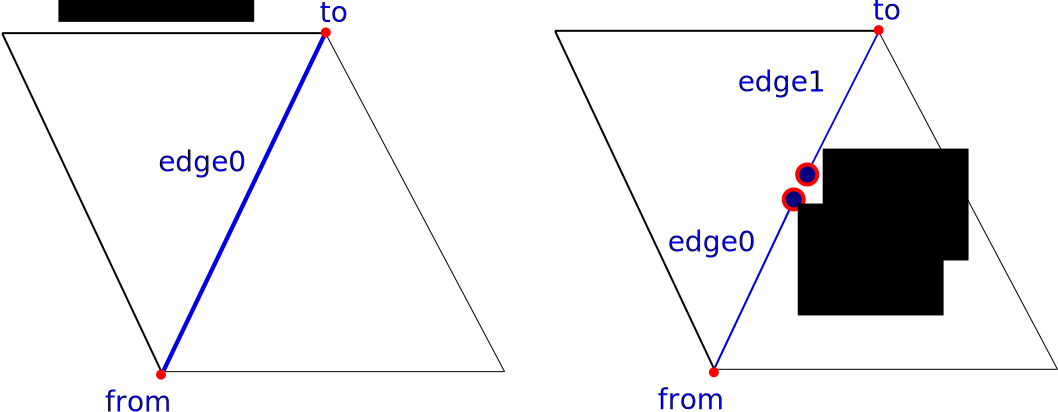
\includegraphics[width=0.8\linewidth]{figures/cutting/splitedge.png}
  \caption{\label{fig:splitedge}
  {Top: The edge to be splitted before the splitting operation described in algorithm \ref{alg:edgesplit}. 
  Bottom: Splitting an edge produces a pair of new half-edges $he2$ and $he3$ which connect to the original half-edges $he0$ and $he1$
  at the point of intersection.}
}
\end{figure}

Iterating over all incoming half-edges can also be easily done using our structure as shown in \ref{alg:incomingHalfEdges}:

\begin{algorithm}[H]
\caption{Iterating over incoming half-edges. Input to this algorithm is an index to a node, output is a list
of half-edges.}
\label{alg:incomingHalfEdges}
\begin{algorithmic}[1]	
  \STATE $outHE \gets outgoingHalfEdge(node)$
  \STATE $first \gets oppositeHalfEdge(outHE)$
  \STATE $current \gets first$
  
  \REPEAT
    \STATE $incomingHE.append(current)$
    \STATE $current = oppositeHalfEdge(nextHalfEdge(current))$
  \UNTIL{$current == first$}
  
  \RETURN $incomingHE$
\end{algorithmic}
\end{algorithm}

A similar algorithm can be written to iterate over outgoing half-edges. Upon topological modification, events are generated to 
notify cutting algorithms of the internal changes in the mesh structure. This is also useful for debugging and evaluation purposes and
can be logged for accounting the sequence of changes made to the original mesh. The events include removal and/or insertions of edges,
 faces and elements.


In the next section we describe the cutting algorithm which is based on the halfedge data structure presented in this section.

\section{Cutting Algorithm}
Our cutting algorithm follows the same strategy presented by Ganovelli \etal \cite{Ganovelli2000} which suggests use of lookup tables to 
handle different configurations. We also applied the optimizations suggested by
Steinemann and Mor \etal \cite{Steinemann, Mor2000} to have minimal new elements added to the mesh under cut. 
The first stage in our cutting algorithm is detecting the cut sweep-surface. The input to this stage is the cut trajectory which is a list of points
that the scalpel passed through in Euclidean space. The cut trajectory is not collected until the axis-aligned bounding box of the cutting tool intersects
with that of the tissue. The tissue bounding box is expanded to rule out the boundary cases where the surface of the model contacts with its own bounding 
box. In such cases the scalpel might miss the surface if the bounding box test fails to detect the initial contact. 

\begin{figure}[H]
  \centering
  % the following command controls the width of the embedded PS file
  % (relative to the width of the current column)
  \includegraphics[width=0.8\linewidth]{figures/cutting/sweep_surface.png}
  \caption{\label{fig:sweepsurf}
  {The cut trajectory in blue and the sweep-surface shown in pink. The scalpel passes through a single 
  tetrahedral element for cutting.}
}
\end{figure}

\subsection{Edge Intersections}
Using a GPU kernel function the intersection of the sweep-surface and all the edges of the model are computed. 
The input to this stage is the list of edges of the model and 4 points defining the sweep-surface quadrilateral. 
Since the intersection of a triangle and a line segment is faster to compute than a quadrilateral, we 
use two intersection tests per each edge to figure out wether the segment is splitted or not. The implementation
of our edge triangle intersection follows the Ray-Triangle intersection test given in \cite{RTR3}.

Listing below shows the prototype of the kernel function in OpenCL:

\begin{lstlisting}[frame=single]
//Computes the intersection of edges and sweepsurface
float sweepSurfEdgeIntersections(unsigned int countEdges,
			         __global float4* edgeBuffer,
				 __global float4 sweepSurface[4],
				 __global float4* outIntersections,
				 __global unsigned int* outIndices,
				 __global unsigned int* outSplitted);
\end{lstlisting}
		     
\begin{algorithm}[H]
\caption{\textit{EdgeIntersections}: The kernel function that computes intersections of edges 
and the sweep-surface. The prototype of the kernel follows the listing above and the algorithm here represents one 
thread of the execution. }
\label{alg:edgeIntersections}
\begin{algorithmic}[1]	
  \IF{$dim.x \geq countEdges$}
  \STATE return
  \ENDIF
  \STATE $outSplitted[dim.x] \gets 0$
  \STATE $tri0 \gets triangle(0, 1, 2, sweepSurface)$
  \STATE $tri1 \gets triangle(0, 2, 3, sweepSurface)$
  \STATE $edge0 \gets edgeBuffer[dim.x * 2]$
  \STATE $edge1 \gets edgeBuffer[dim.x * 2 + 1]$
  \STATE $res \gets IntersectSegmentTri(edge0, edge1, tri0, p)$
  \IF{$res = 0$}
  \STATE $res = IntersectSegmentTri(edge0, edge1, tri1, p)$
  \ENDIF
  \IF{$res \neq 0$}
  \STATE $outIntersections[dim.x] \gets p$
  \STATE $outIndices[dim.x] \gets dim.x$
  \STATE $outSplitted[dim.x] \gets 1$
  \ENDIF
  
\end{algorithmic}
\end{algorithm}

Similar to our GPU polygonization method in section \ref{sec:surfextraction}, a prefix-sum operator is applied to 
the $outSplitted$ array to identify the offsets within the output to store the intersection points. 
The final output of this stage is a list of intersection points and the associated edge indices:

\begin{algorithm}[H]
\caption{\textit{ScanEdgeIntersections}: Counts and compacts edge-intersections using
prefix-sum scan primitives. The inputs to this stage are the outputs of algorithm \ref{alg:edgeIntersections} }

\label{alg:compactEdgeIntersections}
\begin{algorithmic}[1]	
  \STATE $scannedSplitted \gets prefixSumScan(outSplitted)$
  \STATE $total \gets scannedSplitted[countEdges-1]$
  \STATE $compactedIndices.allocateGPUMemory(total, sizeof(uint))$
  \STATE $compactedIntersections.allocateGPUMemory(total, sizeof(float4))$
  \STATE $compactedIndices \gets compactScan(outSplitted, scannedSplitted, outIndices)$
  \STATE $compactedIntersections \gets compactScan(outSplitted, scannedSplitted, outIntersections)$
\end{algorithmic}
\end{algorithm}

The results stored in $outIntersections$ and $outIndices$ arrays are compacted and stored into separate arrays.

\subsection{GPU Compaction}
Dynamic arrays residing in the GPU memory can be compacted to produce the final output.
As depicted in figure \ref{fig:compactkernel} an active array is supplied to the compaction kernel 
to identify the valid slots in the input. The process starts by performing a sum-scan operator over the active array
to produce the offsets that basically guide the location in the output array to store valid elements from the input. 

Upon each thread of execution, the validity of the current array element is checked against the \textit{active} array 
and the final location to store the element is determined by the \textit{offset} array. The final output is the 
compacted version of the input array.


\begin{figure}[H]
  \centering
  % the following command controls the width of the embedded PS file
  % (relative to the width of the current column)
  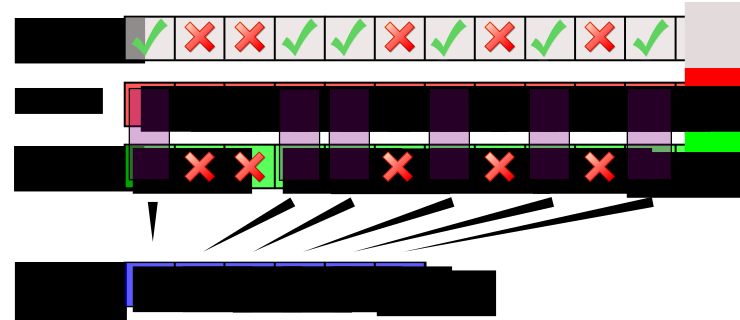
\includegraphics[width=0.8\linewidth]{figures/cutting/compactkernel.png}
  \caption{\label{fig:compactkernel}
  {The array compaction process: Inputs are active, scanned active or offset arrays and the input array of elements to be compacted.
  Output is the single compacted array of elements.}
}
\end{figure}

\subsection{Preserve existing faces}


%The main contribution of our cutting method is the GPU-accelerations applied to the cutting process to support interactive topological 
%modifications and the post processing step that supports smoothness of the cuts in case of complex tissues. 

